\documentclass{scrartcl}
\usepackage[utf8]{inputenc}
%\usepackage[T1]{fontenc}
\usepackage[a4paper, left=2.5cm, right=2.5cm, top=2.5cm, bottom=4cm]{geometry}
\usepackage[english]{babel}
\usepackage{amsmath, amsthm, amssymb, amstext}
\usepackage{listings}
\usepackage{color}
\usepackage{graphicx}
\usepackage{xparse}
\usepackage{fancyhdr}
\usepackage{algorithmicx}
\usepackage{algpseudocode}
\usepackage{algorithm}
\usepackage{parskip}
\usepackage[table]{xcolor}
\usepackage{tabularx}
\usepackage{enumerate}
\usepackage{enumitem}
%\usepackage{minted}
\usepackage {tikz}
\usetikzlibrary{positioning}

\pagestyle{fancy}


\rhead{{\newcommand\and\\\getauthors}}
\author{Felix Bühler\\2973410 \and Clemens Lieb\\3130838 \and Steffen Wonner\\2862123 \and Fabian Bühler\\2953320}
\lhead{\textbf\gettitle}
\title{\gettitle}
\chead{\getsubtitle}
\subtitle{\getsubtitle}

\addtolength{\headheight}{2\baselineskip}
\renewcommand{\headrulewidth}{0pt}

\newcommand{\gettitle}{Distributed systems I\\Winter Term 2019/20}
\newcommand{\getsubtitle}{G2T1 – Assignment 4 (theoretical part)}
\newcommand{\getauthors}{Felix Bühler \and Clemens Lieb \and Steffen Wonner \and Fabian Bühler}
\setlength{\headheight}{53pt}

\begin{document}
\maketitle

\section*{1 - Global State}
\subsection*{a)}
$C_{1}$: $e_{11}$ $e_{21}$ $e_{31}$ $e_{12}$ $e_{22}$\\
$C_{2}$: $e_{11}$ $e_{21}$ $e_{31}$ $e_{12}$ $e_{22}$ $e_{41}$

\subsection*{b)}
\begin{enumerate}[label=(\roman*)]
\item
The inequation give true for all states that can follow the first one given independant on how many states lie between them. To make sure that the other state lies on level L+1 you can either check if any other state lies between them or check the timestamps. The stamp of the prosess with tha last event has to be 1 higher than in the other state.
\item
$S_{30}$ -> $S_{31}$ = true
$S_{30}$ -> $S_{32}$ = true
$S_{30}$ -> $S_{42}$ = true

$S_{31}$ -> $S_{32}$ = true
$S_{32}$ -> $S_{42}$ = true
So $S_{32}$ and $S_{42}$ are not on level L+1, because $S_{31}$ lies between them and $S_{30}$.\\
You either have to check the timestamps (not given) or check all other states if they lie between $S_{30}$ and $S_{31}$. Non of them do so $S_{31}$ is on level l+1 of $S_{30}$.
\end{enumerate}
\subsection*{c)}

\tikzstyle{nofill}=[rectangle,draw, align=center]
\tikzstyle{green}=[rectangle,draw,fill=green!50,align=center]
\tikzstyle{blue}=[rectangle,draw,fill=blue!50,align=center]
\tikzstyle{both}=[rectangle,draw,fill=red!50!,align=center]

\begin{figure}[!ht]
\centering
\begin{tikzpicture}[auto,node distance=1.5cm]
\node[green] (s00) {$ S_{00} $ \\ $ x_1 = 0 $ \\ $ x_2 = 0 $};

\node[both] (s10) [below left = of s00] {$ S_{10} $ \\ $ x_1 = 10 $ \\ $ x_2 = 0 $};

\node[both] (s20) [below left = of s10] {$ S_{20} $ \\ $ x_1 = 5 $ \\ $ x_2 = 0 $};
\node[green] (s11) [below right = of s10] {$ S_{11} $ \\ $ x_1 = 10 $ \\ $ x_2 = 20 $};

\node[both] (s30) [below left = of s20] {$ S_{30} $ \\ $ x_1 = 15 $ \\ $ x_2 = 0 $};
\node[green] (s21) [below left = of s11] {$ S_{21} $ \\ $ x_1 = 5 $ \\ $ x_2 = 20 $};
\node[green] (s12) [below right = of s11] {$ S_{12} $ \\ $ x_1 = 10 $ \\ $ x_2 = 30 $};

\node[nofill] (s31) [below left = of s21] {$ S_{31} $ \\ $ x_1 = 15 $ \\ $ x_2 = 20 $};
\node[green] (s22) [below left = of s12] {$ S_{22} $ \\ $ x_1 = 5 $ \\ $ x_2 = 30 $};

\node[green] (s32) [below left = of s22] {$ S_{32} $ \\ $ x_1 = 15 $ \\ $ x_2 = 30 $};

\node[both] (s42) [below left = of s32] {$ S_{42} $ \\ $ x_1 = 55 $ \\ $ x_2 = 30 $};

\node[both] (s52) [below left = of s42] {$ S_{52} $ \\ $ x_1 = 60 $ \\ $ x_2 = 30 $};

\node[both] (s53) [below right = of s52] {$ S_{53} $ \\ $ x_1 = 60 $ \\ $ x_2 = 13 $};

\path (s10) edge node {} (s00);

\path (s10) edge node {} (s11);
\path (s10) edge node {} (s20);

\path (s11) edge node {} (s21);
\path (s20) edge node {} (s21);
\path (s20) edge node {} (s30);
\path (s11) edge node {} (s12);

\path (s30) edge node {} (s31);
\path (s21) edge node {} (s31);
\path (s21) edge node {} (s22);
\path (s12) edge node {} (s22);


\path (s31) edge node {} (s32);
\path (s22) edge node {} (s32);

\path (s32) edge node {} (s42);

\path (s42) edge node {} (s52);

\path (s52) edge node {} (s53);
\end{tikzpicture}
\caption{solution for 1.c)}
\end{figure}

\subsection*{d)}
\begin{itemize}
	\item $ \phi_{1} = (x_{2} - x_{1}) = 5 $\\
	$ \Rightarrow (\neg\phi_{1}) $ marked in \textcolor{blue}{blue}
	\item $ \phi_{2} = (x_{2} - x_{1}) \leq 5 $ and $ (x_{2} - x_{1}) > 0 $\\
	$ \Rightarrow (\phi_{2}) $ marked in \textcolor{green}{green}
	\item if they fulfill $ (\neg\phi_{1}) $ and $ (\phi_{2}) $ marked in \textcolor{red}{red}
\end{itemize}

\begin{enumerate}
	\item safety condition $ \neg\phi_{1} $ is not fulfilled in the state $ S_{31} $ and thereby not fulfilled.
	\item liveness condition $ \phi_{2} $ is fulfilled in the end and thereby fulfilled.
\end{enumerate}
\section*{2 - Transaction Processing}
\subsection*{a)}
The conflicting operation pairs are:
\[\{(w_1[u], w_3[u]), (r_1[y], w_2[y]), (r_3[y], w_2[y]), (r_2[x], w_3[x])\}\]

\subsection*{b)}

\begin{figure}[ht!]
\begin{tikzpicture}
    \node[draw, circle] at (0, 0)    (T1) {\(T_1\)};
    \node[draw, circle] at (5, 0)    (T2) {\(T_2\)};
    \node[draw, circle] at (2.5,2.5) (T3) {\(T_3\)};

    \draw[->]
        (T1) edge node[above,sloped] {\(w_1[y] \to r_2[y]\)} (T2)
        (T2) edge node[above,sloped] {\(w_2[z] \to w_3[z]\)} (T3)
        (T3) edge node[above,sloped] {\(w_3[y] \to r_1[y]\)} (T1);
\end{tikzpicture}
\caption{Serialization Graph for History \(H_1\)}
\label{fig:sg_h1}
\end{figure}

It's clear that the serialization graph shown in Figure \ref{fig:sg_h1} contains a cycle, as such \(H_1\) is not serializable.\\~\\

\begin{figure}[ht!]
\begin{tikzpicture}
    \node[draw, circle] at (0, 0)    (T1) {\(T_1\)};
    \node[draw, circle] at (5, 0)    (T2) {\(T_2\)};
    \node[draw, circle] at (2.5,2.5) (T3) {\(T_3\)};

    \draw[->]
        (T2) edge node[above,sloped] {\(r_2[y] \to w_1[y]\)} (T1)
        (T3) edge node[above,sloped] {\(r_3[x] \to w_1[x]\)} (T1)
        (T3) edge node[above,sloped] {\parbox[c]{2.5cm}{\(r_3[x] \to w_2[x] \\ w_3[u] \to w_2[u]\)}} (T2);
\end{tikzpicture}
\caption{Serialization Graph for History \(H_2\)}
\label{fig:sg_h2}
\end{figure}

The serialization graph shown in Figure \ref{fig:sg_h2} does not contain a cycle, which would imply that \(H_2\) is serializable.\\
Unfortunately \(H_2\) is not a correct history as it does not specify the order or the conflicting operations \(w_1[x], w_2[x]\).



\section*{3 - Two-Phase Locking}

\begin{itemize}
    \item[\(H_1\):] could be generated by 2-phase-locking. The shrinking phase for each transaction begins right after the last operation before the commit.

        Execution split for each resource:

        \begin{itemize}
            \item[\(y\):] \(rL_1 \rightarrow r_1 \rightarrow wL_1 \rightarrow w_1 \rightarrow wU_1 \rightarrow rL_2 \rightarrow r_2 \rightarrow c_1 \rightarrow rU_2 \rightarrow c_2 \rightarrow c_3\)
            \item[\(x\):] only read operations $\Rightarrow$ no conflicting locks possible
            \item[\(z\):] only read operations $\Rightarrow$ no conflicting locks possible
            \item[\(w\):] \(c_1 \rightarrow wL_2 \rightarrow w_2 \rightarrow wU_2 \rightarrow c_2 \rightarrow wL_3 \rightarrow w_3 \rightarrow wU_3 \rightarrow c_3\)
        \end{itemize}

    \item[\(H_2\):] is not possible with 2-phase-locking!

        Conflicting excerpt: \(r_1[x] \rightarrow w_2[x] \rightarrow r_1[y]\)

        Either \(T_2\) cannot aquire the write lock for \(w_2[x]\) as \(T_1\) still holds the read lock or \(T_1\) is already in the lock shrinking phase when it wants to execute \(r_1[y]\) (this is the first operation of \(T_1\)on \(y\)) but both transactions commit.

    \item[\(H_3\):] is not possible with 2-phase-locking!

        Conflicting excerpt: \(r_1[y] \rightarrow w_3[y] \rightarrow w_1[z]\)

        Analog situation to \(H_2\). Shrinking for \(T_1\) can only happen after \(w_1[z]\) but \(r_1[y]\) and \(w_3[y]\) are conflicting locks.


\end{itemize}

\end{document}
